%\documentclass[spanish,a4paper]{article}
\documentclass[11pt]{article}
\usepackage[utf8]{inputenc}
\usepackage[a4paper,margin=6em]{geometry}
\usepackage[spanish]{babel}

% Paquetes generales
\usepackage{amsmath}
\usepackage[utf8]{inputenc}%esto permite meter tildes sin el coso
\usepackage[spanish]{babel}
\usepackage{ifthen}
\usepackage{amssymb}
\usepackage{amsmath}
\usepackage{multicol}
\usepackage[absolute]{textpos}
\usepackage{hyperref}
\usepackage{enumitem}
%\usepackage{graphicx}
\usepackage{aed2-tad, aed2-symb, aed2-itef}
\usepackage{algpseudocode}
\usepackage{modulos}
\usepackage{caratula}
\usepackage{float}%este es el que acomoda bien las figures
\usepackage{tikz}
\usetikzlibrary{calc}
\pgfdeclarelayer{bg}
\pgfsetlayers{bg,main}

\newcommand{\linea}{\noindent\rule{12cm}{0.4pt}}

%% **************************************************************************
%
%  Package 'caratula', version 0.5 (para componer caratulas de TPs del DC).
%
%  En caso de dudas, problemas o sugerencias sobre este package escribir a
%  Brian J. Cardiff (bcardif arroba gmail.com).
%  Nico Rosner (nrosner arroba dc.uba.ar).
%
% **************************************************************************

% ----- Informacion sobre el package para el sistema -----------------------

\NeedsTeXFormat{LaTeX2e}
\ProvidesPackage{caratula}[2013/08/04 v0.5 Para componer caratulas de TPs del DC]
\RequirePackage{ifthen}
\usepackage[pdftex]{graphicx}

% ----- Imprimir un mensajito al procesar un .tex que use este package -----

\typeout{Cargando package 'caratula' v0.5 (2013/08/04)}

% ----- Algunas variables --------------------------------------------------

\let\Materia\relax
\let\Submateria\relax
\let\Titulo\relax
\let\Subtitulo\relax
\let\Grupo\relax
\let\Fecha\relax
\let\Logoimagefile\relax
\newcommand{\LabelIntegrantes}{}
\newboolean{showLU}
\newboolean{showEntregas}
\newboolean{showDirectores}

% ----- Comandos para que el usuario defina las variables ------------------

\def\materia#1{\def\Materia{#1}}
\def\submateria#1{\def\Submateria{#1}}
\def\titulo#1{\def\Titulo{#1}}
\def\subtitulo#1{\def\Subtitulo{#1}}
\def\grupo#1{\def\Grupo{#1}}
\def\fecha#1{\def\Fecha{#1}}
\def\logoimagefile#1{\def\Logoimagefile{#1}}

% ----- Token list para los integrantes ------------------------------------

\newtoks\intlist\intlist={}

\newtoks\intlistSinLU\intlistSinLU={}

\newcounter{integrantesCount}
\setcounter{integrantesCount}{0}
\newtoks\intTabNombre\intTabNombre={}
\newtoks\intTabLU\intTabLU={}
\newtoks\intTabEmail\intTabEmail={}

\newcounter{directoresCount}
\setcounter{directoresCount}{0}
\newtoks\direcTabNombre\direcTabNombre={}
\newtoks\direcTabEmail\direcTabEmail={}

% ----- Comando para que el usuario agregue integrantes --------------------

\def\integrante#1#2#3{%
    \intlist=\expandafter{\the\intlist\rule{0pt}{1.2em}#1&#2&\tt #3\\[0.2em]}%
    \intlistSinLU=\expandafter{\the\intlistSinLU\rule{0pt}{1.2em}#1 & \tt #3\\[0.2em]}%
    %
    \ifthenelse{\value{integrantesCount} > 0}{%
        \intTabNombre=\expandafter{\the\intTabNombre & #1}%
        \intTabLU=\expandafter{\the\intTabLU & #2}%
        \intTabEmail=\expandafter{\the\intTabEmail & \tt #3}%
    }{
        \intTabNombre=\expandafter{\the\intTabNombre #1}%
        \intTabLU=\expandafter{\the\intTabLU #2}%
        \intTabEmail=\expandafter{\the\intTabEmail \tt #3}%
    }%
    \addtocounter{integrantesCount}{1}%
}

\def\director#1#2{%
    \ifthenelse{\value{directoresCount} > 0}{%
        \direcTabNombre=\expandafter{\the\direcTabNombre & #1}%
        \direcTabEmail=\expandafter{\the\direcTabEmail & \tt #2}%
    }{
        \direcTabNombre=\expandafter{\the\direcTabNombre #1}%
        \direcTabEmail=\expandafter{\the\direcTabEmail \tt #2}%
    }%
    \addtocounter{directoresCount}{1}%
}

% ----- Macro para generar la tabla de integrantes -------------------------

\newcommand{\tablaIntegrantes}{\ }

\newcommand{\tablaIntegrantesVertical}{%
\ifthenelse{\boolean{showLU}}{%
    \begin{tabular}[t]{| l @{\hspace{4ex}} c @{\hspace{4ex}} l|}
        \hline
        \multicolumn{1}{|c}{\rule{0pt}{1.2em} \LabelIntegrantes} & LU &  \multicolumn{1}{c|}{Correo electr\'onico} \\[0.2em]
        \hline \hline
        \the\intlist
        \hline
    \end{tabular}
}{
    \begin{tabular}[t]{| l @{\hspace{4ex}} @{\hspace{4ex}} l|}
        \hline
        \multicolumn{1}{|c}{\rule{0pt}{1.2em} \LabelIntegrantes} &  \multicolumn{1}{c|}{Correo electr\'onico} \\[0.2em]
        \hline \hline
        \the\intlistSinLU
        \hline
    \end{tabular}
    }%
}

\newcommand{\tablaIntegrantesHorizontal}{%
    \begin{tabular}[t]{ *{\value{integrantesCount}}{c} }
    \the\intTabNombre \\%
\ifthenelse{\boolean{showLU}}{
    \the\intTabLU \\%
}{}
    \the\intTabEmail %
    \end{tabular}%
}

\newcommand{\tablaDirectores}{%
\ifthenelse{\boolean{showDirectores}}{%
	\bigskip
	Directores

	\smallskip
    \begin{tabular}[t]{ *{\value{directoresCount}}{c} }
    \the\direcTabNombre \\%
    \the\direcTabEmail %
    \end{tabular}%
}{}%
}

\newcommand{\tablaEntregas}{%
\ifthenelse{\boolean{showEntregas}}{%
  \bigskip%
  \begin{tabular}[t]{|l p{3.5cm} p{1.5cm}|}%
  \hline%
  \rule{0pt}{1.2em} Instancia & Docente & Nota \\[0.2em] %
  \hline%
  \hline%
  \rule{0pt}{1.2em} Primera entrega & & \\[0.2em] %
  \hline%
  \rule{0pt}{1.2em} Segunda entrega & & \\[0.2em] %
  \hline%
  \end{tabular}%
}{}%
}

% ----- Codigo para manejo de errores --------------------------------------

\def\se{\let\ifsetuperror\iftrue}
\def\ifsetuperror{%
    \let\ifsetuperror\iffalse
    \ifx\Materia\relax\se\errhelp={Te olvidaste de proveer una \materia{}.}\fi
    \ifx\Titulo\relax\se\errhelp={Te olvidaste de proveer un \titulo{}.}\fi
    \edef\mlist{\the\intlist}\ifx\mlist\empty\se%
    \errhelp={Tenes que proveer al menos un \integrante{nombre}{lu}{email}.}\fi
    \expandafter\ifsetuperror}

\def\aftermaketitle{%
  \setcounter{page}{1}
}

% ----- \maketitletxt correspondiente a la versi�n v0.2.1 (texto v0.2 + fecha ) ---------

\def\maketitletxt{%
    \ifsetuperror\errmessage{Faltan datos de la caratula! Ingresar 'h' para mas informacion.}\fi
    \thispagestyle{empty}
    \begin{center}
    \vspace*{\stretch{2}}
    {\LARGE\textbf{\Materia}}\\[1em]
    \ifx\Submateria\relax\else{\Large \Submateria}\\[0.5em]\fi
    \ifx\Fecha\relax\else{\Large \Fecha}\\[0.5em]\fi
    \par\vspace{\stretch{1}}
    {\large Departamento de Computaci\'on}\\[0.5em]
    {\large Facultad de Ciencias Exactas y Naturales}\\[0.5em]
    {\large Universidad de Buenos Aires}
    \par\vspace{\stretch{3}}
    {\Large \textbf{\Titulo}}\\[0.8em]
    {\Large \Subtitulo}
    \par\vspace{\stretch{3}}
    \ifx\Grupo\relax\else\textbf{\Grupo}\par\bigskip\fi
    \tablaIntegrantes
    \end{center}
    \vspace*{\stretch{3}}
    \newpage\aftermaketitle}

% ----- \maketitletxtlogo correspondiente v0.2.1 (texto con fecha y logo) ---------

\def\maketitletxtlogo{%
    \ifsetuperror\errmessage{Faltan datos de la caratula! Ingresar 'h' para mas informacion.}\fi
    \thispagestyle{empty}
    \begin{center}
    \ifx\Logoimagefile\relax\else\includegraphics{\Logoimagefile}\fi \hfill 
\includegraphics{logo_dc.jpg}\\[1em]
    \vspace*{\stretch{2}}
    {\LARGE\textbf{\Materia}}\\[1em]
    \ifx\Submateria\relax\else{\Large \Submateria}\\[0.5em]\fi
    \ifx\Fecha\relax\else{\large \Fecha}\\[0.5em]\fi
    \par\vspace{\stretch{1}}
    {\large Departamento de Computaci\'on}\\[0.5em]
    {\large Facultad de Ciencias Exactas y Naturales}\\[0.5em]
    {\large Universidad de Buenos Aires}
    \par\vspace{\stretch{3}}
    {\Large \textbf{\Titulo}}\\[0.8em]
    {\Large \Subtitulo}
    \par\vspace{\stretch{3}}
    \ifx\Grupo\relax\else\textbf{\Grupo}\par\bigskip\fi
    \tablaIntegrantes
    \end{center}
    \vspace*{\stretch{4}}
    \newpage\aftermaketitle}

% ----- \maketitlegraf correspondiente a la versi�n v0.3 (gr�fica) -------------

\def\maketitlegraf{%
    \ifsetuperror\errmessage{Faltan datos de la caratula! Ingresar 'h' para mas informacion.}\fi
%
    \thispagestyle{empty}

    \ifx\Logoimagefile\relax\else\includegraphics{\Logoimagefile}\fi \hfill 
\includegraphics{logo_dc.jpg}

    \vspace*{.06 \textheight}

    \noindent \textbf{\huge \Titulo}  \medskip \\
    \ifx\Subtitulo\relax\else\noindent\textbf{\large \Subtitulo} \\ \fi%
    \noindent \rule{\textwidth}{1 pt}

    {\noindent\large\Fecha \hspace*\fill \Materia} \\
    \ifx\Submateria\relax\else{\noindent \hspace*\fill \Submateria}\fi%

    \medskip%
    \begin{center}
        \ifx\Grupo\relax\else\textbf{\Grupo}\par\bigskip\fi
        \tablaIntegrantes

        \tablaDirectores

        \tablaEntregas
    \end{center}%
    \vfill%
%
    \begin{minipage}[t]{\textwidth}
        \begin{minipage}[t]{.55 \textwidth}
            
\includegraphics{logo_uba.jpg}
        \end{minipage}%%
        \begin{minipage}[b]{.45 \textwidth}
            \textbf{\textsf{Facultad de Ciencias Exactas y Naturales}} \\
            \textsf{Universidad de Buenos Aires} \\
            {\scriptsize %
            Ciudad Universitaria - (Pabell\'on I/Planta Baja) \\
                Intendente G\"uiraldes 2160 - C1428EGA \\
            Ciudad Aut\'onoma de Buenos Aires - Rep. Argentina \\
                Tel/Fax: (54 11) 4576-3359 \\
            http://www.fcen.uba.ar \\
            }
        \end{minipage}
    \end{minipage}%
%
    \newpage\aftermaketitle}

% ----- Reemplazamos el comando \maketitle de LaTeX con el nuestro ---------
\renewcommand{\maketitle}{\maketitlegraf}

% ----- Dependiendo de las opciones ---------
%
% opciones:
%   txt     : caratula solo texto.
%   txtlogo : caratula txt con logo del DC y del grupo (opcional).
%   graf    : (default) caratula grafica con logo del DC, UBA y del grupo (opcional).
%
\@makeother\*% some package redefined it as a letter (as color.sty)
%
% Layout general de la caratula
%
\DeclareOption{txt}{\renewcommand{\maketitle}{\maketitletxt}}
\DeclareOption{txtlogo}{\renewcommand{\maketitle}{\maketitletxtlogo}}
\DeclareOption{graf}{\renewcommand{\maketitle}{\maketitlegraf}}
%
% Etiqueta Autores o Integrantes
%
\DeclareOption{integrante}{\renewcommand{\LabelIntegrantes}{Integrante}}
\DeclareOption{autor}{\renewcommand{\LabelIntegrantes}{Autor}}
%
% Formato tabla de integrantes
%
\DeclareOption{intVert}{\renewcommand{\tablaIntegrantes}{\tablaIntegrantesVertical}}
\DeclareOption{intHoriz}{\renewcommand{\tablaIntegrantes}{\tablaIntegrantesHorizontal}}
\DeclareOption{conLU}{\setboolean{showLU}{true}}
\DeclareOption{sinLU}{\setboolean{showLU}{false}}
\DeclareOption{conEntregas}{\setboolean{showEntregas}{true}}
\DeclareOption{sinEntregas}{\setboolean{showEntregas}{false}}
\DeclareOption{showDirectores}{\setboolean{showDirectores}{true}}
\DeclareOption{hideDirectores}{\setboolean{showDirectores}{false}}
%
% Opciones predeterminadas
%
\ExecuteOptions{intVert}%
\ExecuteOptions{graf}%
\ExecuteOptions{integrante}%
\ExecuteOptions{conLU}%
\ExecuteOptions{hideDirectores}%
\ExecuteOptions{sinEntregas}%
%
\ProcessOptions\relax

\begin{document}


\titulo{Trabajo Pr\'{a}ctico}
\subtitulo{}

\fecha{\today}

\materia{Algoritmos y Estructuras de Datos 3}
\grupo{}

\integrante{Zabaleta, Agustín}{449/13}{mfosco2005@yahoo.com.ar}
\integrante{Jessica, Fernandez de La Vega}{449/13}{mfosco2005@yahoo.com.ar}
\integrante{chiqui, El}{449/13}{mfosco2005@yahoo.com.ar}
\integrante{Fosco, Martín Esteban}{449/13}{mfosco2005@yahoo.com.ar}

\maketitle

\thispagestyle{empty}
\vspace{3cm}
\tableofcontents
\newpage
\vfill

\begin{abstract}
En este trabajo se implementaron algoritmos que proporcionen soluciones a los tres problemas recibidos. A continuación se describen los problemas, dando ejemplos, y luego se describen en detalle los algoritmos que los resuelven.
\end{abstract}

\newpage



\section{El Telégrafo}

\subsection{El Problema}

\subsubsection{Introducción}
Se plantea en este caso el problema de, dados:
\begin{itemize}

\item Una cantidad de kilómetros de cable para un ramal.

\item Una cierta cantidad $n$ de ciudades en un orden determinado, identificadas por la cantidad de kilómetros que las separan de la capital (además de la capital, que se encuentra implícita en todas las sucesiones de ciudades propuestas).

\end{itemize}


Hallar la mayor cantidad posible de ciudades que se puedan conectar con dicho cable sin cortarlo, en otras palabras: optimizar el uso del cable para conectar la mayor cantidad de ciudades consecutivas.
De este resultado óptimo se quiere obtener como resultado cuántas ciudades se pudieron conectar.

Es necesario además que el algoritmo funcione con orden de complejidad O($n$).


\subsubsection{Ejemplos}

A modo de ejemplo de qué plantea el problema, y sus soluciones, se observan casos:\\ \\

\noindent\rule{13cm}{0.4pt}


Dados 3 km de cable y las siguientes ciudades: (identificadas por la cantidad de km que las separan de la capital).\\

\begin{figure}[H]
\begin{tikzpicture}
  \hspace*{1.5cm}
  
  \node [fill=gray!30] (0) at (0,0) { 0 };
  \node [fill=gray!30] (2) at (1,0) { 1 };
  \node [fill=gray!30] (3) at (2,0) { 2 };
  \node [fill=gray!30] (6) at (6,0) { 6 };
  \node [fill=gray!30] (7) at (7,0) { 7 };
  \node [fill=gray!30] (10) at (10,0) { 10 };
  
  \begin{pgfonlayer}{bg}    % select the background layer
      \draw (0) (10);
  \end{pgfonlayer}

\end{tikzpicture}
\end{figure}

En este caso, lo ideal sería conectar las ciudades 0, 2, 3 entre sí, ya que la cantidad de cable es suficiente y en total conseguiría conectar 3 ciudades, en otros lugares conseguiría conectar menos ciudades:\\

\begin{figure}[H]
\begin{tikzpicture}
  \hspace*{1.5cm}
  
  \node [fill=gray!30] (0) at (0,0) { 0 };
  \node [fill=gray!30] (1) at (1,0) { 1 };
  \node [fill=gray!30] (2) at (2,0) { 2 };
  \node [fill=gray!30] (6) at (6,0) { 6 };
  \node [fill=gray!30] (7) at (7,0) { 7 };
  \node [fill=gray!30] (10) at (10,0) { 10 };
  
  \begin{pgfonlayer}{bg}    % select the background layer
      \hspace*{1.5cm}
      \draw (0)--(3) (10);
  \end{pgfonlayer}

\end{tikzpicture}
\end{figure}

Nota: \textbf{NO} se pueden conectar las ciudades 0-3 y las 6-7 de la siguiente manera:

\begin{figure}[H]
\begin{tikzpicture}
  \hspace*{1.5cm}
  
  \node [fill=gray!30] (0) at (0,0) { 0 };
  \node [fill=gray!30] (1) at (1,0) { 1 };
  \node [fill=gray!30] (2) at (2,0) { 2 };
  \node [fill=gray!30] (6) at (6,0) { 6 };
  \node [fill=gray!30] (7) at (7,0) { 7 };
  \node [fill=gray!30] (10) at (10,0) { 10 };
  
  \begin{pgfonlayer}{bg}    % select the background layer
      \hspace*{1.5cm}
      \draw (0)--(3) (6)--(7) (10);
  \end{pgfonlayer}

\end{tikzpicture}
\end{figure}

Si bien se pueden conseguir 5 ciudades de esta manera, los intervalos no son consecutivos, sino que están separados, es necesario que sea distribuido en sólo un intervalo.

\newpage

\linea


Dados 10 km de cable y las siguientes ciudades: \\

\begin{figure}[H]
\begin{tikzpicture}
  \hspace*{0.5cm}
  \node [fill=gray!30] (0) at (0,0) { 0 };
  \node [fill=gray!30] (2) at (1,0) { 2 };
  \node [fill=gray!30] (6) at (3,0) { 6 };
  \node [fill=gray!30] (8) at (4,0) { 8 };
  \node [fill=gray!30] (14) at (7,0) { 14 };
  \node [fill=gray!30] (16) at (8,0) { 16 };
  \node [fill=gray!30] (20) at (10,0) { 20 };
  \node [fill=gray!30] (22) at (11,0) { 22 };
  
  \begin{pgfonlayer}{bg}    % select the background layer
      \draw (0) (22);
  \end{pgfonlayer}
\end{tikzpicture}
\end{figure}

En este caso existen varias respuestas posibles, todas con el mismo resultado, se pueden conseguir 4 ciudades como máximo de las siguientes maneras:

\begin{figure}[H]
\begin{tikzpicture}
  \hspace*{0.5cm}
  \node [fill=gray!30] (0) at (0,0) { 0 };
  \node [fill=gray!30] (2) at (1,0) { 2 };
  \node [fill=gray!30] (6) at (3,0) { 6 };
  \node [fill=gray!30] (8) at (4,0) { 8 };
  \node [fill=gray!30] (14) at (7,0) { 14 };
  \node [fill=gray!30] (16) at (8,0) { 16 };
  \node [fill=gray!30] (20) at (10,0) { 20 };
  \node [fill=gray!30] (22) at (11,0) { 22 };
  
  \begin{pgfonlayer}{bg}    % select the background layer
      \hspace*{0.5cm}
      \draw (0)--(8) (22);
  \end{pgfonlayer}
\end{tikzpicture}
\end{figure}

\begin{figure}[H]
\begin{tikzpicture}
  \hspace*{0.5cm}
  \node [fill=gray!30] (0) at (0,0) { 0 };
  \node [fill=gray!30] (2) at (1,0) { 2 };
  \node [fill=gray!30] (6) at (3,0) { 6 };
  \node [fill=gray!30] (8) at (4,0) { 8 };
  \node [fill=gray!30] (14) at (7,0) { 14 };
  \node [fill=gray!30] (16) at (8,0) { 16 };
  \node [fill=gray!30] (20) at (10,0) { 20 };
  \node [fill=gray!30] (22) at (11,0) { 22 };
  
  \begin{pgfonlayer}{bg}    % select the background layer
      \hspace*{0.5cm}
      \draw (0) (6)--(16) (22);
  \end{pgfonlayer}
\end{tikzpicture}
\end{figure}

\begin{figure}[H]
\begin{tikzpicture}
  \hspace*{0.5cm}
  \node [fill=gray!30] (0) at (0,0) { 0 };
  \node [fill=gray!30] (2) at (1,0) { 2 };
  \node [fill=gray!30] (6) at (3,0) { 6 };
  \node [fill=gray!30] (8) at (4,0) { 8 };
  \node [fill=gray!30] (14) at (7,0) { 14 };
  \node [fill=gray!30] (16) at (8,0) { 16 };
  \node [fill=gray!30] (20) at (10,0) { 20 };
  \node [fill=gray!30] (22) at (11,0) { 22 };
  
  \begin{pgfonlayer}{bg}    % select the background layer
      \hspace*{0.5cm}
      \draw (0) (14)--(22);
  \end{pgfonlayer}
\end{tikzpicture}
\end{figure}

Como el algoritmo debe retornar sólo el máximo de ciudades, cualquiera de los intervalos que tomemos para conectar con nuestros cables servirán a nuestro propósito.

En definitiva, la respuesta será 4 ciudades.

\linea

\subsection{El Algoritmo}


\newpage


\section{A Medias}

\subsection{El Problema}

\subsection{El Algoritmo}



\newpage


\section{Girls Scouts}

\subsection{El Problema}
 \subsubsection{Introducción}
Se plantea en este caso el problema de, dados:
\begin{itemize}

\item Un conjunto de niñas exploradoras.

\item Las relaciones de amistad entre ellas, es decir, para cada niña, sus amigas dentro del grupo de exploradoras.
\end{itemize}

Hallar la manera de sentarlas en una ronda, de manera tal que las niñas que son amigas, estén a una distancia mínima. Formalmente dicho, se pide que la sumatoria de las distancias entre todos los pares de amigas, sea la mínima. Como resultado, se debe devolver la distancia máxima entre los pares de amigas de la ronda, junto con la misma. 

El algoritmo debe funcionar con orden de complejidad estrictamente mejor que O($e^{e}  a^{2}$), donde \textbf{e} es la cantidad de exploradoras, y \textbf{a} es la cantidad de amistades.

\subsubsection{Ejemplos}

\vspace{2mm}
\textbf{Ejemplo 1}
\vspace{2mm}

A modo de ejemplo de qué plantea el problema, y sus soluciones, se observan casos:\\ 

Dado el grupo de exploradoras conformado por \{a, b, c, d, e\}, y sus respectivas amistades: 

\begin{center}
\{\{a,b\}\{a,c\}\{a,d\}\{a,e\}\{b,c\}\{b,d\}\{b,e\}\{c,d\}\{c,e\}\}
\end{center}

Notar que utilizamos un conjunto de conjuntos para ejemplificar las amistades porque estas son simétricas, lo que quiere
decir que si \textbf{a} es amiga de \textbf{b} entonces \textbf{b} es amiga de \textbf{a}. Cada una de las
amistades tiene su correspondiente distancia en la ronda. Por ejemplo, una posible manera de sentarlas es:

\begin{figure}[H]
\begin{center}
  \begin{tikzpicture}
    \hspace*{0.5cm}
    \node [fill=gray!30] (a) at (0,0) { a };
    \node [fill=gray!30] (b) at (2,2) { b };
    \node [fill=gray!30] (c) at (1,4) { c };
    \node [fill=gray!30] (d) at (-1,4) { d };
    \node [fill=gray!30] (e) at (-2,2) { e };
    
    \begin{pgfonlayer}{bg}    % select the background layer
      %%        \draw (0) (a)--(b) (22);
      %%        \draw (0) (e)--(b);
    \end{pgfonlayer}
  \end{tikzpicture}
\end{center}
\end{figure}

Donde la sumatoria de las distancias entre todos los pares de amigas en esta ronda es 14.
\begin{itemize}
  \item d(a,b) = 1   \ \ \ \inlineitem d(a,c) = 2 \ \ \ \inlineitem d(a,d) = 2
  \item d(a,e) = 1   \ \ \ \inlineitem d(b,c) = 1 \ \ \ \inlineitem d(b,d) = 2
  \item d(b,e) = 2   \ \ \ \inlineitem d(c,d) = 1 \ \ \ \inlineitem d(c,e) = 2
\end{itemize}

Donde d(x,y) es la distancia entre x e y.

Como el problema nos pedía la ronda cuya distancia entre los pares de amigas sea la mínima, podemos 
ver intuitivamente como esta ronda no es óptima ya que \textbf{d} y \textbf{e} no son amigas, sin embargo
están sentadas juntas (a distancia 1). Como en este caso la cantidad mínima de amistades que tiene
una exploradora es 3, no puede haber una solución óptima donde sentemos juntas a dos que no son amigas.
Podemos ver como al separarlas obtenemos una ronda mejor (cuya distancia total entre todos los
pares de amigas es menor):

\begin{figure}[H]
\begin{center}
  \begin{tikzpicture}
    \hspace*{0.5cm}
    \node [fill=gray!30] (a) at (0,0) { a };
    \node [fill=gray!30] (b) at (2,2) { b };
    \node [fill=gray!30] (c) at (1,4) { d };
    \node [fill=gray!30] (d) at (-1,4) { c };
    \node [fill=gray!30] (e) at (-2,2) { e };
    
    \begin{pgfonlayer}{bg}    % select the background layer
      %%        \draw (0) (a)--(b) (22);
      %%        \draw (0) (e)--(b);
    \end{pgfonlayer}
  \end{tikzpicture}
\end{center}
\end{figure}

\begin{itemize}
  \item d(a,b) = 1   \ \ \ \inlineitem d(a,c) = 2 \ \ \ \inlineitem d(a,d) = 2
  \item d(a,e) = 1   \ \ \ \inlineitem d(b,c) = 2 \ \ \ \inlineitem d(b,d) = 1
  \item d(b,e) = 2   \ \ \ \inlineitem d(c,d) = 1 \ \ \ \inlineitem d(c,e) = 1
\end{itemize}

Por ende, la sumatoria de las distancias entre todos los pares de amigas en esta ronda es 13.
\vspace{2mm}
\textbf{Ejemplo 2}\\
\vspace{2mm}
Dado el grupo de exploradoras conformado por \{a, b, c\} donde ninguna es amiga de otra. En este caso tenemos que 
cualquier manera de sentar al grupo de exploradoras es solución al problema, porque no hay ninguna restricción al respecto.

Como todas las posibles permutaciones de la ronda son soluciones posibles, al ser \{a, b, c\} la menor lexicográficamente, 
es la solución al problema.

\subsection{Estructuras}

En esta sección discutiremos las posibles estructuras de representación que podrían ser utilizadas
para la resolución de este problema, y justificaremos nuestra elección.

Para el conjunto de exploradoras, lo importante es que queremos modelar una ronda. Sin importar
qué utilicemos efectivamente para representarla, consideramos de suma importancia (por el uso de abstracción,
declaratividad, y modularización del problema) utilizar una clase hecha por nosotros que modele el 
comportamiento de la ronda.

Posibles estructuras que se pueden utilizar para implementar las rondas son: 
\begin{itemize}
\item Lista simple o doblemente enlazada
\item Lista circular
\item Arreglo
\item Vector
\end{itemize}
La estructura que utilizamos para resolver el problema de representación de la Ronda 
fue un Vector que modela el comportamiento de una 
lista circular a través de las operaciones provistas por la clase Ronda. Por ejemplo [a,b,c,d,e] es una 
posible representación de la ronda donde, teniendo en cuenta el hecho de que es circular,
se puede observar la distancia entre \textbf{a} y \textbf{e} es 1 en vez de 4 porque del último se puede llegar al primero.

Por el otro lado sus respectivas amistades se pueden representar, por ejemplo, con:
\begin{itemize}
\item Matriz de booleanos (1 indica amistad, 0 no).
\item Diccionario con claves exploradoras y significado sus amigas.
\item Lista de listas.
\item Conjunto de conjuntos.
\end{itemize}
La estructura que utilizamos para resolver el problema de representación de las amistades fue un conjunto de
conjuntos, ya que nos interesó representar la simetría entre las amistades y que, por ejemplo, la amistad 
\{a,b\} es igual a \{b,a\}.

Además, nuestro contexto de uso (del cual se desprende la complejidad) no 
nos impuso ninguna restricción que no permitiera el uso de alguna de las estructuras mencionadas previamente.

\subsection{El Algoritmo}

\subsubsection{Complejidad}

En esta sección mostraremos un pseudocódigo de nuestra implementación, junto con su explicación y justificación
de complejidad.

La idea del algoritmo utilizado para resolver el problema fue, dado que tenemos que encontrar la ronda 
que mínimiza la sumatoria de la distancias, generar todas las posibles permutaciones de la ronda de exploradoras
y elegir la óptima. Para comparar entre dos rondas cuál es mejor a la solución del problema, 
recorremos el conjunto de amistades y para cada una de ellas sumamos su distancia en un acumulador. Luego, nos quedamos
con aquella para la que dicha sumatoria sea menor.

Sólo por un tema de notación, al conjunto de conjuntos de char lo renombramos como bigSet, para hacer menos 
engorroso el código.
\\ \\
\noindent\makebox[\linewidth]{\rule{17cm}{0.4pt}}
\algoritmo{rondaOptima}{in/out rondaRes : Tupla(Ronda\, int),in/out exploradoras : Ronda,in amistades : bigSet}{res : string}{
  \Var{n : int}
  \complejidad{O(1)}
  \State $n \larr exploradoras.cantidad()$
  \complejidad{O(1)}
  \If{(amistades.size() $\neq$ 0 $\wedge$ amistades.size() $\neq$ $\frac{n*(n-1)}{2}$)}
  \complejidad{O(1)}
  \State $permutaciones(rondaRes, exploradoras, 0, amistades)$
  \complejidad{O($e!*e*a$)}
  \Else
  \State $\Pi_0{(rondaRes)}.ordenar()$
  \complejidad{O($e^2$)}
  \EndIf
  \Var{dist: int}
  \complejidad{O(1)}
  \State $dist\larr \Pi_0{(rondaRes)}.maxDistAmistades(amistades)$
  \complejidad{O($e*a$)}
  \State $res.append(dist)$
  \complejidad{O(1)}
  \State $res.append(" ")$
  \complejidad{O(1)}
  \Var{i: int}
  \complejidad{O(1)}
  \For {i = 0 \textbf{to} $\Pi_0{(rondaRes)}.cantidad()$}
  \complejidad{O($e^{2}$)}
  \State $res.push\_back(\Pi_0{(rondaRes)}.exploradoraEnPos(i))$
  \complejidad{O($e$)}
  \EndFor
} {O($e!*e*a + e*a + e^2$)}

\vspace{1mm}
Nota: $\Pi_0$ y $\Pi_1$ son utilizados para referirse al primer y segundo elemento de las tuplas.

\vspace{3mm}
\begin{center}
\textbf{Explicación y justificación de complejidad} \\ 
\end{center} 

La complejidad del algoritmo es O($e!*e*a + e*a + e^{2}$).

Observamos primero la suma entre ($e!*e*a + e^{2}$)
\begin{itemize}
\item Como $e! = (e*(e-1)*(e-2)*...*1) > e \\ \implies $ $e \in$ O($e!$). \\ Luego, podemos escribir a 
  ($e!*e*a + e^2$) = ($e *(e!*a + e)$) $\in$ O($e *(e!*a + e)$) \\ $\implies$ O($e*max(e!*a, e)$) \\ lo cual, por lo demostrado anteriormente, es equivalente a O($e!*a*e$)
\item Como ($e!*e*a + e*a$) = ($e*a (e! + 1)$) $\in$ O($(e!*e*a)$)
\end{itemize}
Luego, la complejidad total del algoritmo es O($e!*e*a)$).

Nuestro algoritmo cumple con la cota de complejidad provista por la cátedra ya que:
\begin{itemize}
  \item Como $e! = (e*(e-1)*(e-2)*...*3*2*1) < e^{e-1}$ \\ $\implies$ $e! < e^{e-1}$ \\ $\implies$ $e!*e < e^{e-1}*e 
    = e^{e}$ \\ $\implies$ $e! \in$ O($e^e$) \\
    Luego, como $e! < e^e$ y $a$ $\in$ \mathbb{N}\\ $\implies$ $e!*a < e^e*a < e^e*a^2$
\end{itemize}
Por lo cual, demostramos que la complejidad del algoritmo es O($e!*e*a$) $\in$ O($e^e*a^2$).
Como la complejidad de las funciones \textbf{permutaciones} 
y \textbf{maxDistAmistades} las justificaremos con su debido código, en esta parte explicaremos el resto del 
algoritmo. 

Utilizamos las operaciones \textbf{append} y \textbf{push\_back} que cumplen la misma función en cuanto a que
concatenan al final del string el string o caracter pasado por parámetro, pero por problema de tipos, 
utilizamos las dos en los distintos casos. Ambas operaciones son lineales en la cantidad de elementos del nuevo string concatenado.
Las primeras dos concatenaciones mediante la función \textbf{append} al resultado cuestan O(1) ya que, al 
tener solo dos elementos, esas operaciones son de costo constante.

Luego, el ciclo \textbf{for} que itera sobre el conjunto de exploradoras resultante cicla $e$ veces. En cada
iteración se llama a la función \textbf{push\_back} que le concatena al string el nuevo caracter pasado por parámetro.
En total el ciclo cuesta:

\begin{center}
$\sum\limits_{i=2}^e i = \frac{e*(e-1)}{2} - 1 \in O(e^2)$
\end{center}

Por último, las complejidades de \textbf{exploradoraEnPos} y \textbf{cantidad} son constantes ya que están
directamente implementadas con el operator $[]$ y la función $size()$ de la clase Vector de c++.

Ahora pasaremos a demostrar las complejidades de los algoritmos auxiliares.
\\ \\
\noindent\makebox[\linewidth]{\rule{17cm}{0.4pt}}
\algoritmo{permutaciones}{in/out rondaRes : Tupla(Ronda int),in/out exploradoras : Ronda,in pos : int,in amistades : bigSet}{}{
\If{(pos == exploradoras.cantidad())}
\complejidad{O(1)}
\Var{sumaDists : int}
\complejidad{O(1)}
\State $sumaDists \larr exploradoras.sumaDistancias(amistades)$
\complejidad{O($e*a$)}
\If{(sumaDists $< \Pi_0(rondaRes)$)}
\complejidad{O(1)}
\State $\Pi_0(rondaRes) \larr exploradoras$
\complejidad{O($e$)}
\State $\Pi_1(rondaRes) \larr sumaDists$
\complejidad{O(1)}
\EndIf
\If{((sumaDists == $\Pi_0(rondaRes)) \wedge (exploradoras < \Pi_0(rondaRes)$))}
\complejidad{O($e$)}
\State $\Pi_0(rondaRes) \larr exploradoras$
\complejidad{O($e$)}
\EndIf
\Else
\Var{i : int}
\complejidad{O(1)}
\For{(i = 0 \textbf{to} exploradoras.cantidad())}
\State $exploradoras.swap(pos, i)$
\complejidad{O(1)}
%  \If{exploradoras.exploradoraEnPos(pos, i)}
\State $permutaciones(rondaRes, exploradoras, pos+1, amistades)$
\complejidad{O(1)}
\State $exploradoras.swap(pos, i)$
\complejidad{O(1)}
\EndFor
\EndIf
} {O($e*a$)}

\vspace{3mm}
\begin{center}
\textbf{Explicación y justificación de complejidad} \\ 
\end{center} 

La idea del algoritmo es ir generando todas las permutaciones posibles del conjunto de exploradoras y, en el 
caso base, quedarse con la secuencia de exploradoras cuya sumatoria de distancias entre 
amigas es menor. En caso de que sean iguales, se considera como menor a la menor lexicográficamente. 

Para analizar la complejidad del algoritmo es necesario ver cuántas llamadas recursivas realiza.
\begin{itemize}
\item Cuando pos = 0 (su valor inicial), el algoritmo realiza $e$ llamadas recursivas.
\item Cuando pos = 1 el algoritmo realiza $e-1$ llamadas recursivas.
\item Cuando pos = n el algoritmo realiza $e-n$ llamadas recursivas.
\end{itemize}

Lo cual, al generalizar nos queda la recurrencia de la manera:

\vspace{1mm}

\[ T(e) = 
  \begin{cases} 
    e * T(e-1) & \mbox{si} \ e \ \neq \mbox{1} \\
    1 & \mbox{si} \ e \ \mbox{= 1} 
  \end{cases}
\]

\vspace{2mm}

Entonces, como hago $e!$  llamadas a una función que tiene orden de complejidada O($e*a$) la complejidad 
total es O($e!*e*a$).

\begin{center}
$T(e) = e * T(e-1) = \prod_{i=1}^{e} i = e! \in O(e!)$
\end{center}

\vspace{5mm}
\noindent\makebox[\linewidth]{\rule{17cm}{0.4pt}}

.
\\
\algoritmo{sumaDistancias}{in/out exploradoras : Ronda,in amistades : bigSet}{res : int}{
\Var{exp1 : char}
\complejidad{O(1)}
\Var{exp2 : char}
\complejidad{O(1)}
\Var{acum : int}
\complejidad{O(1)}
\Var{itA : amistades.CrearIterador()}
\complejidad{O(1)}
\While{itA.siguiente() != NULL}
\complejidad{O($a$)}
\State $exp1 \larr primerElem(itA)$
\complejidad{O(1)}
\State $exp2 \larr segundoElem(itA)$
\complejidad{O(1)}
\State $acum \larr acum + distancia(exploradoras, exp1,exp2)$
\complejidad{O($e$)}
\EndWhile
\State $res \larr acum$
\complejidad{O(1)}
}{O($e*a$)}

\vspace{3mm}
\begin{center}
\textbf{Explicación y justificación de complejidad} \\ 
\end{center} 
La idea del algoritmo es ir recorriendo el conjunto de amistades y, por cada amistad, almacenar el valor de 
su distancia en la ronda en un acumulador.

El ciclo itera $a$ veces ya que cicla sobre todo el conjunto de amistades. Las operaciones que obtiene el 
primer y segundo elemento del conjunto amistad son O(1) ya que el tamaño de ese conjunto está acotado por 
2 (las amistades son de a pares). Luego obtiene la distancia entre las dos exploradoras llamando a la 
función \textbf{distancia} la cual es lineal en la cantidad de exploradoras. Por ende la complejidad
total del ciclo, y de la función, es de orden O($e*a$). \\
\noindent\makebox[\linewidth]{\rule{17cm}{0.4pt}}
.
\\
\algoritmo{distancia}{in exploradoras : Ronda,in exp1 : char,in exp2 : char}{res : int}{
\Var{posExp1 : char}
\complejidad{O(1)}
\Var{posExp2 : char}
\complejidad{O(1)}
\Var{dist1: int}
\complejidad{O(1)}
\Var{dist2: int}
\complejidad{O(1)}
\State $posExp1 \larr encontrarPos(exp1)$
\complejidad{O($e$)}
\State $posExp2 \larr encontrarPos(exp2)$
\complejidad{O($e$)}
\State $dist1 \larr abs(posExp1 - posExp2)$
\complejidad{O(1)}
\State $dist2 \larr exploras.size() - dist1$
\complejidad{O(1)}
\State $res \larr min(dist1, dist2)$
\complejidad{O(1)}
}{O($e$)}

\begin{center}
\textbf{Explicación y justificación de complejidad} \\ 
\end{center} 

La idea del algoritmo es encontrar las posiciones de las exploradoras en la ronda y luego, como modelamos 
una lista circular, tener en cuenta que del primero se puede ir al último. Por eso se busca el mínimo entre
la distancia estándar en cualquier arreglo, y la distancia obtenida cuando se puede ir del primero al último.
Como buscar las posiciones dentro de la ronda de las exploradoras es lineal en la cantidad de exploradoras 
el algoritmo tiene orden de complejidad O($e$).

\noindent\makebox[\linewidth]{\rule{17cm}{0.4pt}}
.\\
\algoritmo{encontrarPos}{in exploradoras : Ronda,in exp : char}{res : int}{
\Var{i : int}
\complejidad{O(1)}
\State $i \larr 0$
\complejidad{O(1)}
\While{i $<$ exploradoras.size()}
\complejidad{O($e$)}
\If{exp == exploradoras[i]}
\complejidad{O(1)}
\State $res \larr i$
\complejidad{O(1)}
\EndIf
\State $i \larr i+1$
\complejidad{O(1)}
\EndWhile
} {O($e$)}

\vspace{3mm}
\begin{center}
\textbf{Explicación y justificación de complejidad} \\ 
\end{center} 

La idea del algoritmo es realizar una búsqueda secuencial en la ronda, la cual es lineal en la cantidad de 
exploradoras, y por ende, el algoritmo tiene orden de complejidad O($e$).

\noindent\makebox[\linewidth]{\rule{17cm}{0.4pt}}
.\\
\algoritmo{maxDistAmistades}{in/out exploradoras : Ronda,in amistades : bigSet}{res : int}{
\Var{exp1 : char}
\complejidad{O(1)}
\Var{exp2 : char}
\complejidad{O(1)}
\Var{acum : int}
\complejidad{O(1)}
\Var{itA : amistades.CrearIterador()}
\complejidad{O(1)}
\While{itA.siguiente() != NULL}
\complejidad{O($a$)}
\State $exp1 \larr primerElem(itA)$
\complejidad{O(1)}
\State $exp2 \larr segundoElem(itA)$
\complejidad{O(1)}
\State $acum \larr max(acum, distancia(exploradoras, exp1,exp2))$
\complejidad{O($e$)}
\EndWhile
\State $res \larr acum$
\complejidad{O(1)}
}{O($e*a$)}

\vspace{3mm}
\begin{center}
\textbf{Explicación y justificación de complejidad} \\ 
\end{center} 

La idea del algoritmo es ir recorriendo el conjunto de amistades y en cada iteración elegir la amistad que está   
a una distancia máxima en la ronda.

El ciclo itera $a$ veces ya que cicla sobre todo el conjunto de amistades. Las operaciones que obtienen el 
primer y segundo elemento del conjunto amistad son O(1) ya que el tamaño de ese conjunto está acotado por 
2 (las amistades son de a pares). Luego obtiene la distancia entre las dos exploradoras llamando a la 
función \textbf{distancia} la cual es lineal en la cantidad de exploradoras. Por ende la complejidad
total del ciclo, y de la función, es O($e*a$). 

\subsubsection{Correctitud}

En esta sección mostraremos que la solución obtenida por el algoritmo es la pedida por el problema. 

El problema pide encontrar la ronda cuya sumatoria de las distancias entre los pares de amigas sea la menor.
Nuesta solución al problema fue calcular todas las posibles permutaciones de la ronda de exploradoras, por lo cual 
exploramos todas las posibles soluciones a la manera de sentar las exploradoras. Para cada solución nos fijamos 
si es la que provee en ese momento de ejecución del algoritmo la menor sumatoria de distancias. Como nuestro 
algoritmo evalúa todo el conjunto de posibles soluciones del problema, y se queda en cada caso base con la mejor,
podemos asegurar que el algoritmo es una solución correcta al problema, que cumple con las postcondiciones.

Existen dos casos especiales en los cuales no es necesario calcular todas las permutaciones del conjunto de exploradoras.
\begin{itemize}
  \item Cuando la cantidad de amistades es nula, es decir, cuando ninguna exploradora es amiga de otra.
  \item Cuando todas las exploradoras son amigas de todas.
\end{itemize}
Para estos dos casos lo único que hay que hacer es ordenar lexicográficamente la ronda de menor a mayor. 
Resultan ser los mejores casos del algoritmo ya que cualquier manera de sentar a las exploradoras 
es una solución posible.

En el primer caso se puede notar que no hay ninguna restricción en cuanto a cómo sentarlas 
ya que no hay necesidad de sentar a ninguna al lado de la otra.

En el segundo caso, como todas las exploradoras 
son amigas entre sí no hay manera de diferir en el resultado. En cualquier permutación posible toda exploradora va a tener al lado suyo 
a dos de sus amigas y como máximo a distancia $\lfloor$ $\frac{e}{2}$ $\rfloor$ de una amiga si $e$ es par, o de 
dos amigas si $e$ es impar. 

Luego, el resultado provisto es la ronda de exploradoras ordenada lexicográficamente, la cual es la solución 
al problema en estos casos.

Podemos saber cuál es el tamaño máximo del conjunto de amistades ya que 
se podría pensar al peor caso de las amistades como un grafo completo, donde todos los vértices (exploradoras) estan
relacionados con todos los otros. Como sabemos que la cantidad total de aristas de un grafo G(V,X) es:

\vspace{3mm}

\begin{center}
$\sum\nolimits_{i \in V}d(i) = 2m$ 
\end{center}

\vspace{3mm}

Donde $V$ es la cantidad de vértices, $d(i)$ su grado, siendo el grado de un vértice la 
cantidad de aristas incidentes a ese él, y $m$ la cantidad de aristas total del grafo. Entonces, como
m sería la cantidad total de amistades y si toda exploradora tiene $e-1$ amigas tenemos que:

\vspace{3mm}

\begin{center}
$m = \frac{\sum\limits_{i=1}^e (e-1)}{2} = \frac{e*(e-1)}{2}$
\end{center}

\vspace{3mm}

Con lo cual sabemos que cuando el conjunto de amistades tiene longitud cero o $m$ podemos afirmar que estamos 
en uno de estos dos casos.





\subsubsection{Finalización}

En esta sección demostraremos que dada cualquier entrada que cumpla con la especificación del problema el 
algoritmo termina. Que una entrada de datos cumpla con la especificación del problema significa que no haya
datos sin sentido. En nuestro caso sería que todas las exploradoras en el conjunto de amistades estén en la  
ronda, y que todas las exploradoras de la ronda estén en el conjunto de amistades (la doble inclusión).

Para demostrar que el algoritmo termina, hay que analizar cuatro partes del mismo:
\begin{itemize}
  \item La llamada a la función \textbf{permutaciones}.
  \item La llamada a la función \textbf{ordenar}.
  \item La llamada a la función \textbf{maxDistAmistades}.
  \item El ciclo \textbf{for} que itera sobre la ronda.
\end{itemize}

La función \textbf{permutaciones} consiste en, de manera recursiva, calcular todas las permutaciones posibles 
de una ronda, es decir, todas las posibles maneras de sentar al grupo de exploradoras.
La función es llamada con un parámetro \textbf{pos} que indica la posición sobre la cual se está realizando 
la permutación actual. Esta variable se inicializa en cero, apuntando así al comienzo de la ronda.

El caso base de la función es cuando ya se terminó de calcular una permutación posible, que equivaldría a 
preguntar si el parámetro \textbf{pos} llegó al final del arreglo. En ese caso se compara la 
permutación calculada con la obtenida previamente en los otros pasos recursivos y, en caso de ser menor, se 
la utiliza como nueva ronda óptima hasta el momento.

El caso recursivo consiste en iterar sobre la ronda de exploradoras desde la posición indicada por \textbf{pos} 
hasta el final de la ronda y, por cada iteración, permutar el elemento indicado por esa iteración con la indicada por 
\textbf{pos} en ese caso recursivo. 
Como en cada iteración se llama recursivamente a la función con \textbf{pos} aumentado en 1, sucede que:

\begin{itemize}
\item Cuando pos = 0 el algoritmo realiza $e$ llamadas recursivas con pos = 1.
\item Cuando pos = 1 el algoritmo realiza $e-1$ llamadas recursivas con pos = 2.
\item Cuando pos = n el algoritmo realiza $e-n$ llamadas recursivas con pos = n+1.
\end{itemize}

Por ende, como podemos ver que en cada paso recursivo se reduce el tamaño del problema al aumentar la variables 
\textbf{pos} en 1, podemos afirmar que eventualmente para todas las ramas del árbol de recursión se llega al caso base.

La función ordenar consiste en ordenar la ronda de menor a mayor utilizando el algoritmo \textbf{insertion sort}.
%Justificar por que funciona insertio sort??

La función \textbf{maxDistAmistades} consiste en iterar sobre el conjunto de amistades y, para cada amistad, 
calcular utilizando una búsqueda secuencial en la ronda de exploradoras la posición de cada una, y su distancia.
Luego, en cada iteración, se guarda la máxima de las distancias calculadas.
Como el algoritmo instancia un iterador que recorre desde el principio hasta el final el conjunto de amistades 
una única vez, podemos asegurar que finaliza.

El \textbf{for} del final del algoritmo finaliza ya que recorre una única vez de manera secuencial la ronda 
de exploradoras resultado.

\subsection{Análisis temporal}

En esta sección mostraremos la eficiencia del algoritmo, y cómo se comporta dependiendo del input. Así distinguiremos 
entre los mejores y peores casos del algoritmo.

El tiempo que tarda en finalizar el algoritmo está estrechamente relacionado con la cantidad de exploradoras, la variable $e$ de nuestro problema. Como nuestro algoritmo está basado en la técnica de backtracking, 
calcula todas las posibles permutaciones de la ronda de exploradoras, lo cual deriva en \textbf{e!} posibles soluciones.
Es por esto que la eficiencia del algoritmo no puede diferir en distintos casos teniendo en cuenta únicamente 
a la variable $e$.

Por otro lado, la variable $a$ representa la cantidad de amistades dentro del conjunto de exploradoras la cual, 
aunque no es completamente independiente de la cantidad de exploradoras, puede hacer variar el tiempo que tarda 
en finalizar el algoritmo. Consideramos entonces dos casos particulares para el mejor caso del algoritmo:
\begin{itemize}
  \item Cuando la cantidad de amistades es nula, es decir, cuando ninguna exploradora es amiga de otra.
  \item Cuando todas las exploradoras son amigas de todas.
\end{itemize}
Estos dos casos resultan ser los mejores casos del algoritmo ya que cualquier manera de sentar a las exploradoras 
es una solución posible. Por ende, lo único que hay que hacer es ordenar el arreglo de menor a mayor. 

Luego, el peor caso del algoritmo se da cuando el conjunto de amistades tiene $\frac{e*(e-1)}{2} - 1$ elementos, 
lo cual representa el caso en el que todas son amigas entre sí, excepto por un par.

Para mostrar de manera más clara las diferencias de rendimiento entre los distintos casos, corrimos varias veces 
el algoritmo calculando el tiempo que tardaba en ejecutarse. Luego tomamos el promedio y lo graficamos, de acuerdo a distintos tamaños de inputs.
Para todos los casos, utilizamos grupos de exploradoras de tamaño 3, 5, y 8: \\

\textbf{Caso mejor}:

      \begin{figure}[h]
        \begin{center}
      %  \advance\leftskip-3cm
      %  \advance\rightskip-3cm
        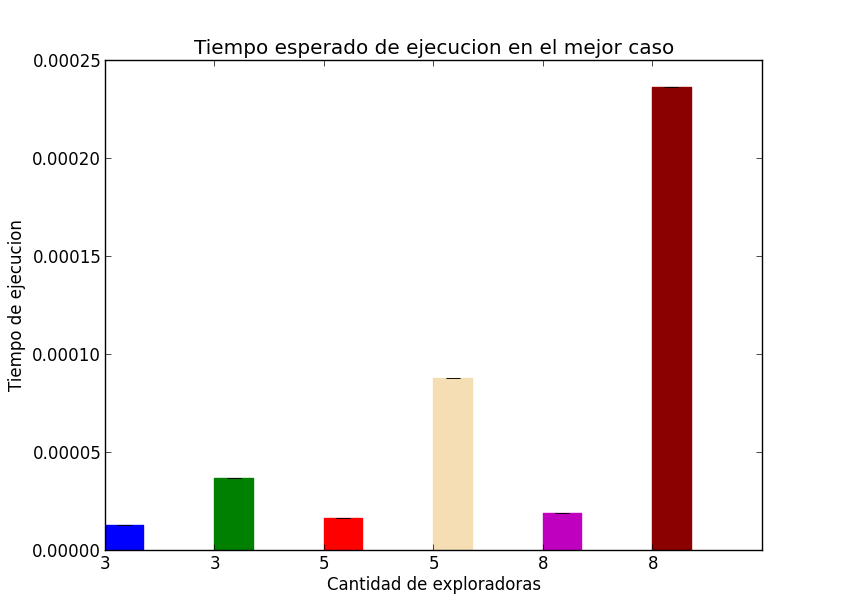
\includegraphics[width=100mm,scale=0.5]{mejorCaso}
        \end{center}
        \end{figure}

Por cada tamaño calculamos el tiempo para los dos mejores casos, a la izquierda cuando el conjunto de amistades es 
nulo, y a la derecha cuando el conjunto de amistades es el más grande posible.
Podemos notar como los casos donde el conjunto de amistades es el máximo el algoritmo tarda más. Esto se debe a que 
al almacenar en memoria más estructuras, la ejecución del algoritmo ralentiza.

\\

\textbf{Caso peor y promedio} \\

Para evaluar el peor caso hicimos ejemplos donde todas las exploradoras eran amigas entre sí, excepto por un par. 
Para el resto de las muestras, realizamos tests sin ninguna intencionalidad. Para generarlos establecimos un conjunto de 
exploradoras y luego generamos de manera pseudoaleatoria el conjunto de amistades. Tomamos un numero random 
usando la función \textbf{rand\_r} y luego le aplicamos módulo tamaño de la ronda para elegir una exploradora al azar. 
Repetimos el procedimiento con la segunda elección hasta que sea distinta de la primera. Iteramos $\frac{e*(e-1)}{2}$
ya que es el la cantidad máxima de posibles amistades.


      \begin{figure}[h]
        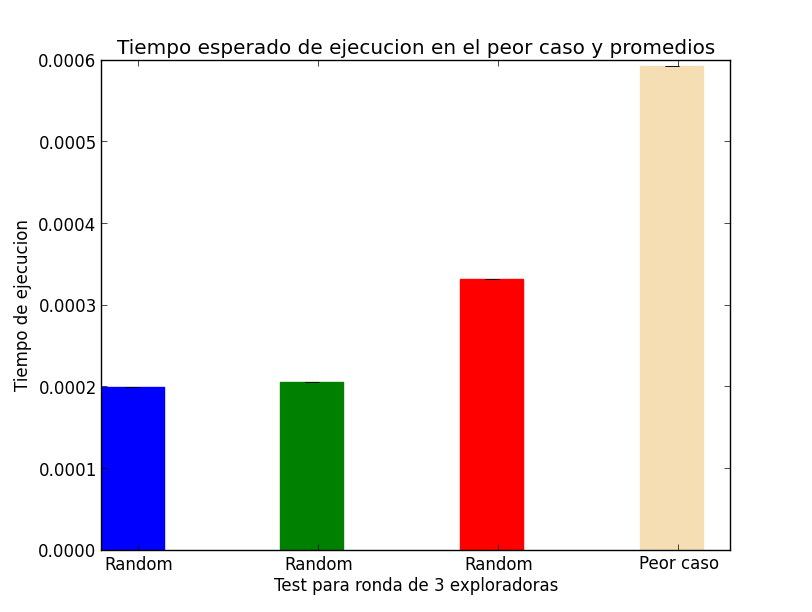
\includegraphics[scale=0.40]{peorCaso3}
        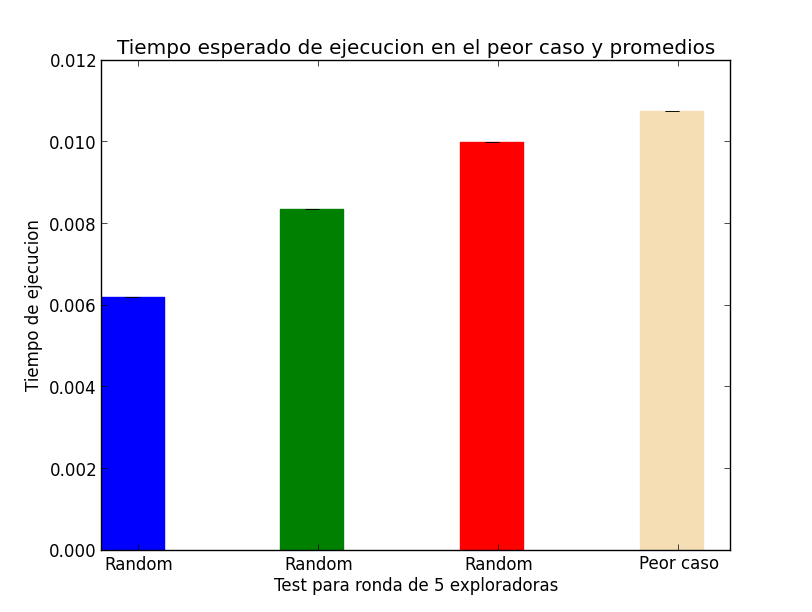
\includegraphics[scale=0.40]{peorCaso5}
        \begin{center}
      %  \advance\leftskip-3cm
      %  \advance\rightskip-3cm
        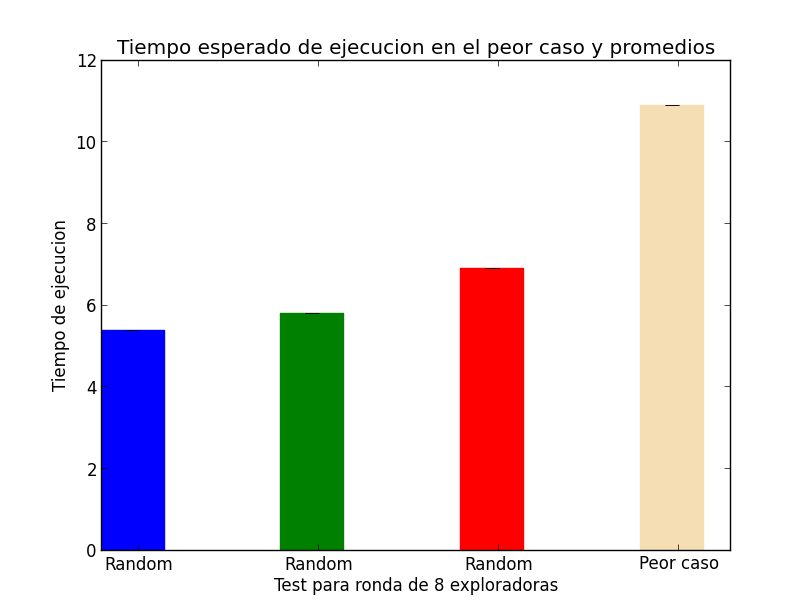
\includegraphics[scale=0.4]{peorCaso8}
        \end{center}
        \end{figure}

Podemos observar cómo el algoritmo difiere temporalmente de manera abrupta al elegir un conjunto de 8 exploradoras
. Esto sucede por la complejidad propia del problema, la cual es factorial en la cantidad de exploradoras.
Por ende, al aumentar levemente la cantidad de exploradoras, el tiempo requerido para finalizar es ampliamente mayor.

Como aclaramos previamente que una vez fijada la cantidad de exploradoras la complejidad temporal del algoritmo 
depende exclusivamente del cardinal del conjunto de amistades, mostramos los siguientes datos:
\begin{itemize}
  \item Para el test con 3 exploradoras el cardinal de amistades es en todos los casos de 1, excepto 
    en el peor caso que es 2.
  \item Para el test con 5 exploradoras el cardinal de amistades es:
    \begin{itemize}
      \item Azul : 5  \ \ \ \ \ \ \inlineitem Verde :  4
      \item Rojo : 8  \ \ \ \ \ \ \inlineitem Rosa  :  9
    \end{itemize}
  \item Para el test con 8 exploradoras el cardinal de amistades es:
    \begin{itemize}
      \item Azul : 13  \ \ \ \ \ \ \inlineitem Verde :  14
      \item Rojo : 15  \ \ \ \ \ \ \inlineitem Rosa  :  28
    \end{itemize}
\end{itemize}

Por ende, una vez fijada la cantidad de exploradoras, podemos observar cómo el tiempo de ejecución del algoritmo 
difiere en base a la cantidad de amistades. 

Como nuestro algoritmo utiliza la técnica de backtracking, la cual consiste en explorar todas las posibles 
soluciones, consideramos utilizar una poda para mejorar el rendimiento del algoritmo. Como el algoritmo pide 
encontrar la ronda que, además de que cumpla la condición de las distancias, también sea la menor lexicográficamente 
se puede utilizar esta información para acotar el espacio de posibles soluciones. En el ejercicio modelamos 
una ronda y lo que nos interesa como resultado es la distancia relativa entre cada amiga, no su posición en la ronda. 
Con sólo explorar las posibles permutaciones que comienzan con la exploradora que es la menor lexicográficamente 
de todo el conjunto es suficiente. Esto sucede porque dada cualquier ronda que no empiece con la menor exploradora, 
se la puede reacomodar a través de rotaciones simples entre las exploradoras contiguas, hasta llegar a una ronda 
cuya distancia entre todas es la misma (ya que no modificamos sus distancias relativas) y es menor lexicográficamente.

Al utilizar esta poda podemos observar como el algoritmo mejora su eficiencia en aproximadamente un 85 porciento: 

      \begin{figure}[h]
        \begin{center}
        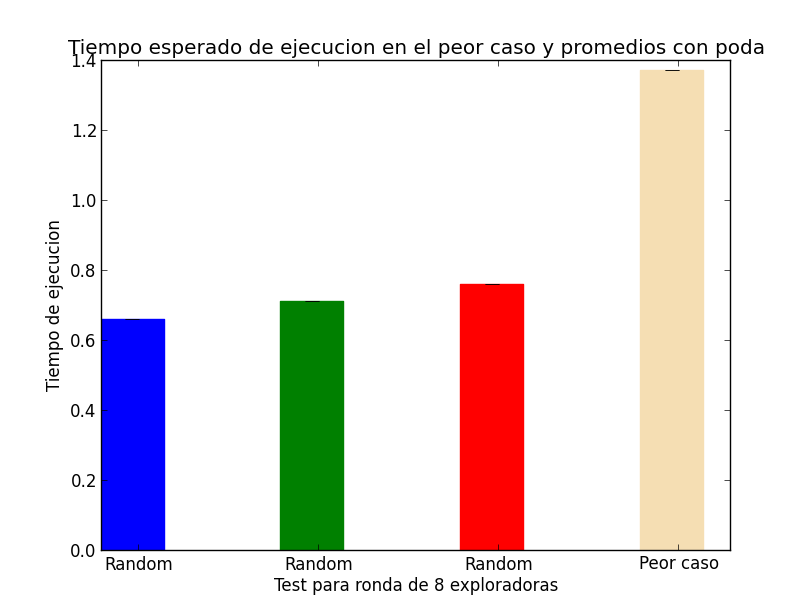
\includegraphics[scale=0.4]{peorCaso8Conpoda}
        \end{center}
        \end{figure}


Falta un poco de explicación aca, o conclusiones y ponerme unidad de medicion de tiempoouu

\end{document}

